
When you're writing CMake files, there are a few core concepts and language features that you need to know about. We won't cover every detail of the language here as CMake's documentation does a pretty good job at this – especially when it comes to being comprehensive. In the following sections, we will provide an overview of the core concepts and language features. Further chapters will dive into the details of different aspects.

The full documentation for the language can be found at \url{https://cmake.org/cmake/help/latest/manual/cmake-language.7.html}.

\subsubsubsection{1.6.1\hspace{0.2cm}The CMake language – a 10,000-feet overview}

CMake uses configuration files called CMakeLists.txt files to determine build specifications. These files are written in a scripting language, often called CMake as well. The language itself is simple and supports variables, string functions, macros, function definitions, and importing other CMake files.

Apart from lists, there is no support for data structures such as structs or classes. But it is this relative simplicity that makes the CMake project inherently maintainable if done properly.

The syntax is based on keywords and whitespace-separated arguments. For example, the following command tells CMake which files are to be added to a library:

\begin{lstlisting}[style=styleCMake]
target_sources(MyLibrary
                PUBLIC include/api.h
                PRIVATE src/internals.cpp src/foo.cpp)
\end{lstlisting}

The PUBLIC and PRIVATE keywords denote the visibility of the files when they're linked against this library and serve as delimiters between the lists of files.

Additionally, the CMake language supports so-called "generator expressions," which are evaluated during build system generation. These are commonly used to specify special information for each build configuration. They will be covered extensively in Chapter 3, Creating a CMake Project.

\hspace*{\fill} \\ %插入空行
\noindent
\textbf{Projects}

CMake organizes the various build artifacts such as libraries, executables, tests, and documentation into projects. There is always exactly one root project, although projects can be encapsulated into each other. As a rule, there should only be one project per CMakeLists.txt file, which means that each project has to have a separate folder in the source directory.

Projects are described like this:

\begin{lstlisting}[style=styleCMake]
project(
  "chapter1"
  VERSION 1.0
  DESCRIPTION "A simple C++ project to demonstrate basic CMake
  usage" LANGUAGES CXX
)
\end{lstlisting}

The current project that's being parsed is stored in the PROJECT\_NAME variable. For the root project, this is also stored in CMAKE\_PROJECT\_NAME, which is useful for determining whether a project is standalone or encapsulated in another. Since version 3.21, there's also a PROJECT\_IS\_TOP\_LEVEL variable to directly determine whether the current project is the top-level project. Additionally, with <PROJECT-NAME>\_IS\_TOP\_LEVEL, you can detect whether a specific project is a top-level project.

The following are some additional variables regarding the projects. All of them can be prefixed with CMAKE\_ to the value for the root project. If they're not defined in the project() directive, the strings are empty:

\begin{itemize}
\item 
PROJECT\_DESCRIPTION: The description string of the project

\item 
PROJECT\_HOMEPAGE\_URL: The URL string for the project

\item 
PROJECT\_VERSION: The full version that's given to the project

\item 
PROJECT\_VERSION\_MAJOR: The first number of the version string

\item 
PROJECT\_VERSION\_MINOR: The second number of the version string

\item 
PROJECT\_VERSION\_PATCH: The third number of the version string

\item 
PROJECT\_VERSION\_TWEAK: The fourth number of the version string
\end{itemize}

Each project has a source and binary directory, and they may be encapsulated in each other. Let's assume that each of the CMakeFiles.txt files in the following example defines a project:

\begin{tcblisting}{commandshell={}}
.
├── CMakeLists.txt #defines project("CMakeBestPractices"...)
├── chapter_1
│      ├── CMakeLists.txt # defines project("Chapter 1"...)
\end{tcblisting}

When parsing the CMakeLists.txt file in the root folder, PROJECT\_NAME and CMAKE\_PROJECT\_NAME will both be CMakeBestPractices. When you're parsing chapter\_1/CMakeLists.txt, the PROJECT\_NAME variable will change to "Chapter\_1" but CMAKE\_PROJECT\_NAME will stay as CMakeBestPractices, as set in the file in the root folder.

Although projects can be nested, it is good practice to write them in a way that they can work standalone. While they may depend on other projects that are lower in the file hierarchy, there should be no need for a project to live as a child of another. It is possible to put multiple calls to project() in the same CMakeLists.txt file, but we discourage this practice as it tends to make projects confusing and hard to maintain. In general, it is better to create a CMakeLists.txt file for each project and organize the structure with subfolders.

This book's GitHub repository, which contains the examples in this book, is organized in a hierarchical way, where each chapter is a separate project that may contain even more projects for different sections and examples.

While each example can be built on its own, you can also build this whole book from the root of the repository.

\hspace*{\fill} \\ %插入空行
\noindent
\textbf{Variables}

Variables are a core part of the CMake language. Variables can be set using the set command and deleted using unset. Variable names are case-sensitive. The following example shows how to set a variable named MYVAR and assign a value of 1234 to it:

\begin{lstlisting}[style=styleCMake]
set(MYVAR "1234")
\end{lstlisting}

To delete the MYVAR variable, we can use unset:

\begin{lstlisting}[style=styleCMake]
unset(MYVAR)
\end{lstlisting}

The general code convention is to write variables in all caps. Internally, variables are always represented as strings.

You can access the value of a variable with the \$ sign and curly brackets:

\begin{lstlisting}[style=styleCMake]
message(STATUS "The content of MYVAR are ${MYVAR}")
\end{lstlisting}

Variable references can even be nested and are evaluated inside out:

\begin{lstlisting}[style=styleCMake]
${outer_${inner_variable}_variable}
\end{lstlisting}

Variables might be scoped in the following way:

\begin{itemize}
\item 
Function scope: Variables that are set inside a function are only visible inside the function.

\item 
Directory scope: Each of the subdirectories in a source tree binds variables and includes any variable bindings from the parent directory

\item 
Persistent cache: Cached variables can be either system- or user-defined. These persist their values over multiple runs.
\end{itemize}

Passing the PARENT\_SCOPE option to set() makes the variable visible in the parent scope.

CMake comes with a wide variety of predefined variables. These are prefixed with CMAKE\_. A full list is available at \url{https://cmake.org/cmake/help/latest/manual/cmake-variables.7.html}.


\hspace*{\fill} \\ %插入空行
\noindent
\textbf{Lists}

Even though CMake stores variables as strings internally, it is possible to work with lists in CMake by splitting values with a semicolon. Lists can be created by either passing multiple unquoted variables to set() or directly as a semicolon-separated string:

\begin{lstlisting}[style=styleCMake]
set(MYLIST abc def ghi)
set(MYLIST "abc;def;ghi")
\end{lstlisting}

Manipulating lists by modifying their contents, reordering, or finding things can be done using the list command. The following code will query MYLIST for the index of the abc value and then retrieve the value and store it in the variable called ABC:

\begin{lstlisting}[style=styleCMake]
list(FIND MYLIST abc ABC_INDEX)
list(GET MYLIST ${ABC_INDEX} ABC)
\end{lstlisting}

To append a value to a list, we can use the APPEND keyword. Here, the xyz value is appended to MYLIST:

\begin{lstlisting}[style=styleCMake]
list(APPEND MYLIST "xyz")
\end{lstlisting}

\hspace*{\fill} \\ %插入空行
\noindent
\textbf{Cached variables and options}

CMake caches some variables so that they run faster in subsequent builds. The variables are stored in CMakeCache.txt files. Usually, you don't have to edit them manually, but they are great for debugging builds that do not behave as expected. 

All the variables that are used to configure the build are cached. To cache a custom variable called ch1\_MYVAR with the foo value, you can use the set command, like this:

\begin{lstlisting}[style=styleCMake]
set(ch1_MYVAR foo CACHE STRING "Variable foo that configures bar")
\end{lstlisting}

Note that cached variables must have a type and a documentation string that provides
a quick summary of them.

Most of the cached variables that are automatically generated are marked as advanced, which means they are hidden from the user in cmake-gui and ccmake by default. To make them visible, they have to be toggled explicitly. If additional cache variables are generated by a CMakeLists.txt file, they can also be hidden by calling the mark\_as\_advanced(MYVAR) command:

\begin{center}
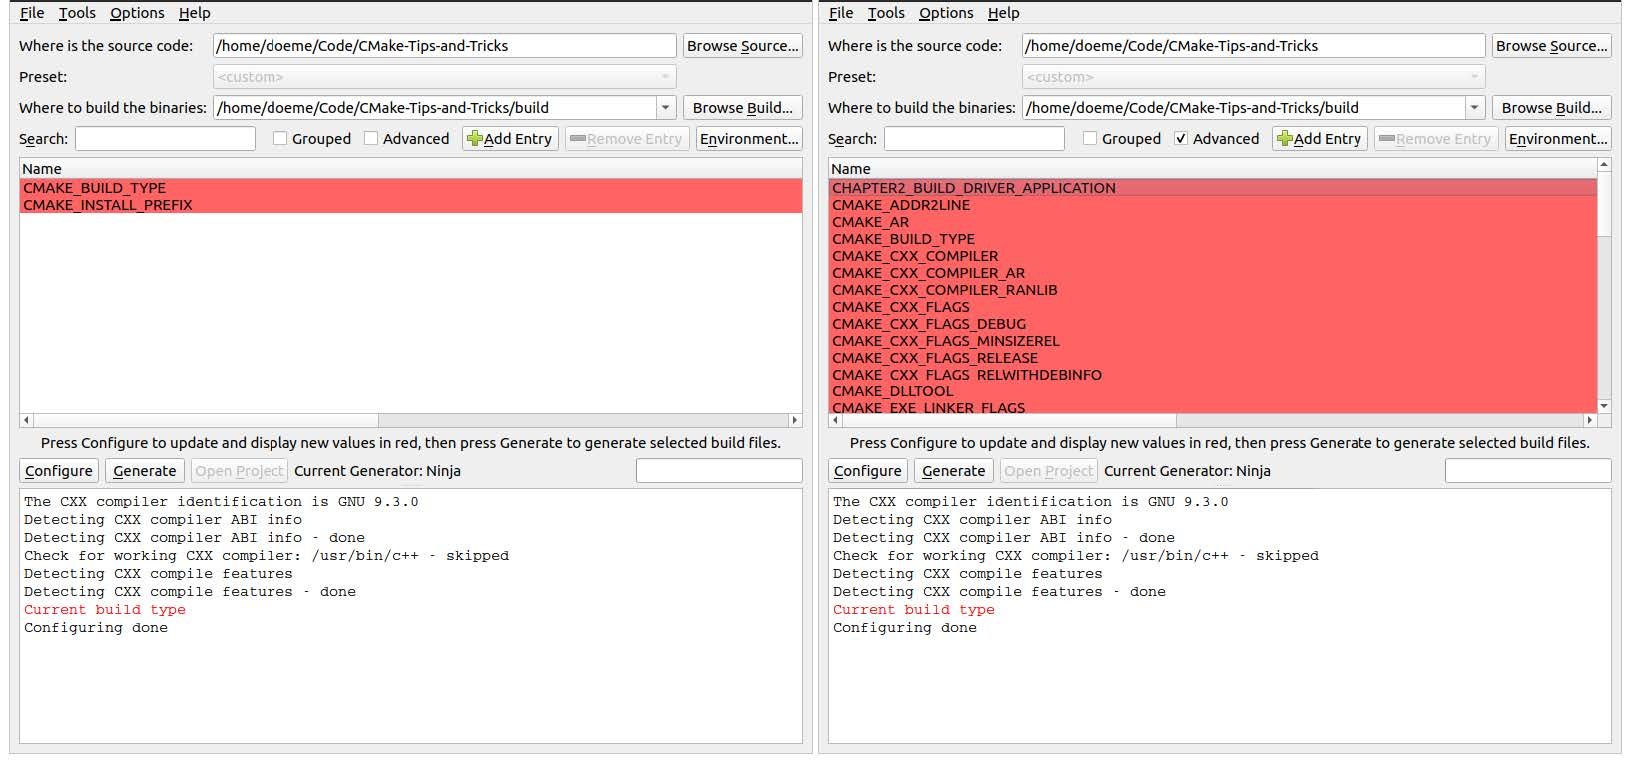
\includegraphics[width=1.\textwidth]{content/1/chapter1/images/4.jpg}\\
Figure 1.4 – Left – cmake-gui does not show variables marked as advanced. Right – Marking the "Advanced" checkbox displays all the variables marked as advanced
\end{center}

As a rule of thumb, any option or variable that the user should change should be marked as advanced. This should happen rarely.

For simple Boolean cache variables, CMake also provides the option keyword. option
has a default value of OFF unless specified otherwise. They can also depend on each other via the CMakeDependentOption module:

\begin{lstlisting}[style=styleCMake]
option(CHAPTER1_PRINT_LANGUAGE_EXAMPLES "Print examples for 
	each language" OFF)
include(CMakeDependentOption)
cmake_dependent_option(CHAPTER1_PRINT_HELLO_WORLD "print a
	greeting from chapter1 " ON CHAPTER1_PRINT_LANGUAGE_EXAMPLES
		ON)
\end{lstlisting}

Options are often a convenient way to specify simple project configuration. They are cache variables of the bool type. If a variable with the same name as the option already exists, a call to option does nothing.

\hspace*{\fill} \\ %插入空行
\noindent
\textbf{Properties}

Properties in CMake are values that are attached to a specific object or scope of CMake, such as a file, target, directory, or test case. Properties can be set or changed by using the set\_property function. To read the value of a property, you can use the get\_property function, which follows a similar pattern. By default, set\_property overwrites the values that are already stored inside a property. Values can be added to the current value by passing APPEND or APPEND\_STRING to set\_property.

The full signature is as follows:

\begin{lstlisting}[style=styleCMake]
set_property(<Scope> <EntityName>
			[APPEND] [APPEND_STRING]
			PROPERTY <propertyName> [<values>])
\end{lstlisting}

The scope specifier may have the following values:

\begin{itemize}
\item 
GLOBAL: Global properties that affect the whole build process.

\item 
DIRECTORY <dir>: Properties that are bound to the current directory or the directories specified in <dir>. These can also be set directly using the set\_directory\_properties command.

\item 
TARGET <targets>: Properties of specific targets. They can also be set using the set\_target\_properties function.

\item 
SOURCE <files>: Applies a property to a list of source files. They can also be set directly using set\_source\_files\_properties. Additionally, there are the SOURCE DIRECTORY and SOURCE TARGET\_DIRECTORY extended options:

\begin{itemize}
\item 
DIRECTORY <dirs>: This sets the property for the source files in the directory's scope. The directory must already be parsed by CMake by either being the current directory or by being added with add\_subdirectory.

\item 
TARGET\_DIRECTORY <targets>: This sets the property to the directory where the specified targets are created. Again, the targets must already exist at the point where the property is set.
\end{itemize}

\item 
INSTALL <files>: This sets the properties for installed files. These can be used to control the behavior of cpack.

\item 
TEST <tests>: This sets the properties for tests. They can also be set directly using set\_test\_properties.

\item 
CACHE <entry>: This sets the properties for cached variables. The most common ones include setting variables as advanced or adding documentation strings to them.
\end{itemize}

The full list of supported properties, sorted by their different entities, can be found at \url{https://cmake.org/cmake/help/latest/manual/cmakeproperties.7.html}.

It is good practice to use direct functions such as set\_target\_properties and set\_test\_properties when modifying properties instead of the more general set\_property command. Using explicit commands avoids making mistakes and confusion between the property names and is generally more readable. There's also the define\_property function, which creates a property without setting the value. We advise that you don't use this as properties should always have a sane default value.

\hspace*{\fill} \\ %插入空行
\noindent
\textbf{Loops and conditions}

Like any programming language, CMake supports conditional and loop blocks. Conditional blocks are in-between if(), elseif(), else(), and endif() statements. Conditions are expressed using various keywords.

Unary keywords are prefixed before the value, as shown here:

\begin{lstlisting}[style=styleCMake]
if(DEFINED MY_VAR)
\end{lstlisting}

The unary keywords to be used in conditions are as follows:

\begin{itemize}
\item 
COMMAND: True if the supplied value is a command

\item 
EXISTS: Checks whether a file or a path exists

\item 
DEFINED: True if the value is a defined variable
\end{itemize}

Additionally, there are unary filesystem conditions:

\begin{itemize}
\item 
EXISTS: True if the passed file or directory exits

\item 
IS\_DIRECTORY: Checks whether the supplied path is a directory

\item 
IS\_SYMLINK: True if the supplied path is a symbolic link

\item 
IS\_ABSOULTE: Checks whether a supplied path is an absolute path
\end{itemize}

Binary tests compare two values and are placed between the values to be compared, like this:

\begin{lstlisting}[style=styleCMake]
if(MYVAR STREQUAL "FOO")
\end{lstlisting}

The binary operators are as follows:

\begin{itemize}
\item 
LESS, GREATER, EQUAL, LESS\_EQUAL, and GREATER\_EQUAL: These compare numeric values.

\item 
STRLESS, STREQUAL, STRGREATER, STRLESS\_EQUAL, and STRGREATER\_EQUAL: These lexicographically compare strings.

\item 
VERSION\_LESS, VERSION\_EQUAL, VERSION\_GREATER, VERSION\_LESS\_EQUAL, and VERSION\_GREATER\_EQUAL: These compare version strings.

\item 
MATCHES: This compares against a regular expression.

\item 
IS\_NEWER\_THAN: Checks which of the two files that passed has been modified recently.

\item 
IS\_NEWER\_THAN: Unfortunately, this is not very precise because if both files have the same timestamp, it also returns true. There is also more confusion because if either of the files is missing, the result is also true.
\end{itemize}

Finally, there's the Boolean OR, AND, and NOT operators.

Loops are either achieved by while() and endwhile() or foreach() and endforeach(). Loops can be terminated using break(); continue() aborts the current iteration and starts the next one immediately.

while loops take the same conditions as an if statement. The following example loops as long as MYVAR is less than 5. Note that to increase the variable, we are using the math() function:

\begin{lstlisting}[style=styleCMake]
set(MYVAR 0)
while(MYVAR LESS "5")
	message(STATUS "Chapter1: MYVAR is '${MYVAR}'")
	math(EXPR MYVAR "${MYVAR}+1")
endwhile()
\end{lstlisting}

In addition to while loops, CMake also knows loops for iterating over lists or ranges:

\begin{lstlisting}[style=styleCMake]
foreach(ITEM IN LISTS MYLIST)
# do something with ${ITEM}
endforeach()
\end{lstlisting}

for loops over a specific range can be created by using the RANGE keyword:

\begin{lstlisting}[style=styleCMake]
foreach(ITEM RANGE 0 10)
# do something with ${ITEM}
endforeach()
\end{lstlisting}

Although the RANGE version of foreach() could work with only a stop variable, it is good practice to always specify both the start and end values.

\hspace*{\fill} \\ %插入空行
\noindent
\textbf{Functions}

Functions are defined by function()/endfunction(). Functions open a new scope for variables, so all the variables that are defined inside are not accessible from the outside unless the PARENT\_SCOPE option is passed to set().

Functions are case-insensitive and are invoked by calling function, followed by parentheses:

\begin{lstlisting}[style=styleCMake]
function(foo ARG1)
# do something
endfunction()
# invoke foo with parameter bar
foo("bar")
\end{lstlisting}

Functions are a great way to make parts of your CMake reusable and often come in handy when you're working on larger projects.

\hspace*{\fill} \\ %插入空行
\noindent
\textbf{Macros}

CMake macros are defined using the macro()/endmacro() commands. They are a
bit like functions, with the difference that in functions, the arguments are true variables, whereas in macros, they are string replacements. This means that all the arguments of a macro must be accessed using curly brackets.

Another difference is that by calling a function, control is transferred to the functions. Macros are executed as if the body of the macro had been pasted into the place of the calling state. This means that macros are not creating scopes regarding variables and control flow. Consequently, it is highly recommended to avoid calling return() in macros as this would stop the scope from executing where the macro is called.

\hspace*{\fill} \\ %插入空行
\noindent
\textbf{Targets}

The build system of CMake is organized as a set of logical targets that correspond to an executable, library, or custom command or artifact, such as documentation or similar.

There are three major ways to create a target in CMake – add\_executable, add\_library, and add\_custom\_target. The first two are used to create executables and static or shared libraries, while the third can contain almost any custom command to be executed.

Targets can be made dependent on each other so that one target has to be built
before another.

It is good practice to work with targets instead of global variables when you're setting properties for build configurations or compiler options. Some of the target properties have visibility modifiers such as PRIVATE, PUBLIC, or INTERFACE to denote which requirements are transitive – that is, which properties have to be "inherited" by a dependent target.


\hspace*{\fill} \\ %插入空行
\noindent
\textbf{Generator expressions}

Generator expressions are small statements that are evaluated during the configuration phase of the build. Most functions allow generator expressions to be used, with a few exceptions. They take the form of \$<OPERATOR:VALUE>, where OPERATOR is applied or compared to VALUE. You can think of generator expressions as small inline if-statements.

In the following example, a generator expression is being used to enable the –Wall compiler flag for my\_target if the compiler is either GCC, Clang, or Apple Clang. Note that GCC is identified as COMPILER\_ID "GNU":

\begin{lstlisting}[style=styleCMake]
target_compile_options(my_target PRIVATE
	"$<$<CXX_COMPILER_ID:GNU,Clang,AppleClang>:-Wall>")
\end{lstlisting}

This example tells CMake to evaluate the CXX\_COMPILER\_ID variable to the commaseparated GNU, Clang, AppleClang list and that if it matches either, append the -Wall option to the target – that is, my\_target. Generator expressions come in very handy for writing platform- and compiler-independent CMake files. 

In addition to querying values, generator expressions can be used to transform strings and lists:

\begin{lstlisting}[style=styleCMake]
$<LOWER_CASE:CMake>
\end{lstlisting}

This will output cmake. 

You can learn more about generator expressions at \url{https://cmake.org/cmake/
help/latest/manual/cmake-generator-expressions.7.html}.

Since CMake supports a variety of build systems, compilers, and linkers, it is often used to build software for different platforms. In the next section, we will learn how CMake can be told which toolchain to use and how to configure the different build types, such as debug or release.

\hspace*{\fill} \\ %插入空行
\noindent
\textbf{CMake policies}

For the top-level CMakeLists.txt file, cmake\_minimum\_required must be called before any call to the project as it also sets which internal policies for CMake are used to build the project.

Policies are used to maintain backward compatibility across multiple CMake releases. They can be configured to use the OLD behavior, which means that cmake behaves backward compatible, or as NEW, which means the new policy is in effect. As each new version will introduce new rules and features, policies will be used to warn you of backwardcompatibility issues. Policies can be disabled or enabled using the cmake\_policy call.

In the following example, the CMP0121 policy has been set to a backward-compatible value. CMP0121 was introduced in CMake version 3.21 and checks whether index variables for the list() commands are in a valid format – that is, whether they are integers:

\begin{lstlisting}[style=styleCMake]
cmake_minimum_required(VERSION 3.21)
cmake_policy(SET CMP0121 OLD)

list(APPEND MYLIST "abc;def;ghi")
list(GET MYLIST "any" OUT_VAR)
\end{lstlisting}

By setting cmake\_policy(SET CMP0121 OLD), backward compatibility is enabled and the preceding code will not produce a warning, despite the access to MYLIST with the "any" index, which is not an integer.

Setting the policy to NEW will throw an error – [build] list index: any is not
a valid index – during the configuration step of CMake.
\
\hspace*{\fill} \\ %插入空行
\begin{tcolorbox}[colback=blue!5!white,colframe=blue!75!black,title=Avoid Setting Single Policies Except When You're Including Legacy Projects]
Generally, policies should be controlled by setting the cmake\_minimum\_required command and not by changing individual policies. The most common use case for changing single policies is when you're including legacy projects as subfolders.
\end{tcolorbox}

So far, we have covered the basic concepts behind the CMake language, which is used to configure build systems. CMake is used to generate build instructions for different kinds of builds and languages. In the next section, we will learn how to specify the compiler to use and how builds can be configured.












